\section{Energetic consistency and resolution sensitivity}
\label{suppsec:consistency}

\subsection{Global energy-balance audit}

For each converged simulation, the signed relative imbalance between power input and viscous dissipation is
\begin{equation}
\varepsilon_E = \frac{P^*-D^*}{D^*}\times 100\%.
\end{equation}
The defect is negative in every case ($P^*<D^*$), between $-1.98\%$ and $-2.17\%$ in magnitude at $N=384$, and it decreases with grid refinement as a first-order (in $1/N$) discretisation error rather than saturating: at $Re=400$, $n=2$, $\alpha=0$ it is $-6.20\%$ ($N=128$), $-3.20\%$ ($N=256$), and $-2.04\%$ ($N=384$), whose ratios $1.94$ and $1.57$ are close to the $2$ and $1.5$ expected for an error proportional to the mesh spacing. It is not an iterative-convergence error, since the velocity change at the final iteration is at or below $9.9\times10^{-9}$ in every case. Because the residual decays as $O(1/N)$, it is a resolution-limited defect of the absolute integrals rather than a fixed estimator offset. It measures the mismatch between the injected power and the computed dissipation; it does not by itself bound the error on $D^*$, and no grid-independent claim is made for the absolute integrals. The matched contrasts (differences of same-grid states) are instead stable to better than $1\%$ (Section~\ref{suppsec:consistency}). Table~\ref{supptab:balance} reports $\varepsilon_E$ for each case at $N=384$.

\begin{table}[!htbp]
\centering
\caption{Energy-balance audit at $N=384$. $\varepsilon_E = |P^*-D^*|/D^* \times 100\%$.}
\label{supptab:balance}
\begin{tabular}{@{}cccc@{}}
\hline
$Re$ & $n$ & $\alpha$ & $\varepsilon_E$ [\%] \\
\hline
$100$  & $2$ & $0.0$  & $1.976$ \\
$100$  & $4$ & $0.0$  & $1.977$ \\
$100$  & $2$ & $0.1$  & $1.976$ \\
$100$  & $4$ & $0.1$  & $1.977$ \\
$100$  & $6$ & $0.0$  & $1.977$ \\
$100$  & $6$ & $0.1$  & $1.977$ \\
$100$  & $8$ & $0.0$  & $1.977$ \\
$100$  & $8$ & $0.1$  & $1.977$ \\
$400$  & $2$ & $0.0$  & $2.041$ \\
$400$  & $4$ & $0.0$  & $2.038$ \\
$400$  & $6$ & $0.0$  & $2.039$ \\
$400$  & $8$ & $0.0$  & $2.040$ \\
$400$  & $2$ & $0.1$  & $2.051$ \\
$400$  & $4$ & $0.1$  & $2.051$ \\
$400$  & $6$ & $0.1$  & $2.051$ \\
$400$  & $8$ & $0.1$  & $2.051$ \\
$1000$ & $2$ & $0.0$  & $2.140$ \\
$1000$ & $4$ & $0.0$  & $2.129$ \\
$1000$ & $6$ & $0.0$  & $2.133$ \\
$1000$ & $8$ & $0.0$  & $2.134$ \\
$1000$ & $2$ & $0.1$  & $2.168$ \\
$1000$ & $4$ & $0.1$  & $2.166$ \\
$1000$ & $6$ & $0.1$  & $2.167$ \\
$1000$ & $8$ & $0.1$  & $2.168$ \\
\hline
\end{tabular}
\end{table}

\begin{table}[!htbp]
\centering
\caption{Energy-balance audit at $N=512$ for the six supplementary cases ($Re=400$ and $Re=1000$, $\alpha=0$ only). $\varepsilon_E = |P^*-D^*|/D^* \times 100\%$.}
\label{supptab:balance512}
\begin{tabular}{@{}ccccc@{}}
\hline
$Re$ & $n$ & $\alpha$ & $\varepsilon_E$ [\%] & iters \\
\hline
$400$  & $2$ & $0.0$  & $1.456$ & $534\,000$ \\
$400$  & $4$ & $0.0$  & $1.454$ & $500\,000$ \\
$1000$ & $2$ & $0.0$  & $1.478$ & $894\,000$ \\
$1000$ & $4$ & $0.0$  & $1.471$ & $1\,178\,000$ \\
$1000$ & $6$ & $0.0$  & $1.474$ & $1\,198\,000$ \\
$1000$ & $8$ & $0.0$  & $1.475$ & $1\,202\,000$ \\
\hline
\end{tabular}
\end{table}

The $N=512$ cases exhibit slightly lower imbalance ($\varepsilon_E \approx 1.45$--$1.48\%$) than their $N=384$ counterparts ($\varepsilon_E \approx 2.04$--$2.17\%$), consistent with the $O(1/N)$ decay of the discretization error. All six cases converged to residuals below $10^{-8}$, with iteration counts between $500\,000$ and $1\,202\,000$.

\subsection{Discrepancy between power- and dissipation-based contrasts}

The agreement between the power-based and dissipation-based estimates of the same contrast is quantified by $\delta_{IP/ID} = 100|I_P/I_D-1|$. At $N=384$ for the transition $(2,4)$, $\alpha=0$, the values are $3.14\%$ ($Re=100$), $1.04\%$ ($Re=400$), and $1.91\%$ ($Re=1000$). For $(4,6)$ at $Re=400$ the discrepancy rises to $10.3\%$, and for $(6,8)$ it is not meaningful because both contrasts are of order $10^{-4}\%$ and their ratio is dominated by cancellation. These values indicate that the two independent routes to the dominant contrast are consistent at this resolution. For the trailing transitions at $Re=1000$, where both contrasts are resolved, the discrepancy is $40.4\%$ for $(4,6)$ ($I_D=+0.0103\%$, $I_P=+0.0062\%$) and $15.6\%$ for $(6,8)$ ($I_D=-0.0037\%$, $I_P=-0.0043\%$); the two estimators still agree in sign for $(6,8)$ but the ratio is not a precision indicator at these magnitudes. At $\alpha=0.1$ and $Re=1000$ the same two transitions give $4.7\%$ and $8.1\%$. This estimator consistency is distinct from the grid-sensitivity analysis: agreement between $I_P$ and $I_D$ at $N=384$ does not imply that the contrast itself is grid-converged.

\subsection{Resolution sensitivity}

At $\alpha=0$ the primary contrast takes the values $I_D(2,4)=0.02161\%$, $0.02195\%$, $0.02178\%$ at $Re=100$; $0.32251\%$, $0.32462\%$, $0.32488\%$, $0.32485\%$ at $Re=400$; and $0.57758\%$, $0.58769\%$, $0.59087\%$, $0.59178\%$ at $Re=1000$ (values at $N=128$, $256$, $384$, $512$; $N=512$ available only at $Re=400$ and $Re=1000$), the target relaxation time being held fixed per Reynolds number. Between $N=256$ and $N=384$ the relative changes are $-0.73\%$ ($Re=100$), $+0.08\%$ ($Re=400$), and $+0.54\%$ ($Re=1000$). The sequence is monotone in $N$ at $Re=400$ and $Re=1000$; at $Re=100$ it is not monotone at the fourth significant figure, but the total span over $N=128$--$384$ is only $3.4\times10^{-4}$ percentage points ($1.6\%$ of the contrast). The contrast is therefore stable to within a few percent of its value over the full $N=128$--$512$ range at all three Reynolds numbers, with full spans of $2.4\times10^{-3}$~pp ($Re=400$) and $1.4\times10^{-2}$~pp ($Re=1000$).

The absolute dissipation is less well converged. For $n=2$, $\alpha=0$, $D^*$ changes by $+0.79\%$ ($Re=100$), $+0.78\%$ ($Re=400$), and $+0.93\%$ ($Re=1000$) between $N=256$ and $N=384$. These changes are larger than those of the contrast, which reflects the partial cancellation of common discretization error in the paired difference. No claim of grid-independent absolute energetics is made. The conservative numerical uncertainties on $I_D(2,4)$ quoted in the main text ($3.4\times10^{-4}$, $2.4\times10^{-3}$, and $1.4\times10^{-2}$ percentage points at $Re = 100$, $400$, and $1000$) are the spans of $I_D(2,4)$ over $N = 128$--$512$ reported in Table~\ref{supptab:contrasts}; they are upper bounds, since the sequence is monotone in $N$ at $Re = 400$ and $Re = 1000$.

At $Re=1000$ the full exponent sequence is resolved at $N=384$: $(2,4)=+0.5909\%$, $(4,6)=+0.0103\%$, $(6,8)=-0.0037\%$. The $N=512$ data at $Re=1000$ confirm the monotonicity of the $(2,4)$ contrast ($+0.592\%$ at $N=512$) and strengthen the negative sign of the $(6,8)$ transition ($-0.0036\%$ at $N=512$). Unlike the $Re=400$ trailing transitions, these two lie well above their own $N=128$--$512$ spans: $(4,6)$ takes $+0.01074\%$, $+0.01058\%$, $+0.01033\%$, $+0.01005\%$ and $(6,8)$ takes $-0.00371\%$, $-0.00360\%$, $-0.00371\%$, $-0.00364\%$ at $N=128$, $256$, $384$, $512$, i.e.\ spans of $6.9\times10^{-4}$ and $1.1\times10^{-4}$ percentage points, each more than twenty times smaller than the corresponding magnitude, and the sign of $(6,8)$ is the same on all four grids. The negative trailing contrast is therefore a resolved Reynolds-dependent effect and not a resolution artefact; it is also insensitive to the amplitude tested, $\alpha=0.1$ giving $-0.0052\%$ with a span of $5.5\times10^{-4}$ percentage points. At $Re=400$ the same $(6,8)$ transition lies inside its own span ($+0.00006\%$ against $1.1\times10^{-4}$) and changes sign between $N=128$ and $N=256$, which is why it is quoted there only as an upper bound.
\begin{figure}[!htbp]
\centering
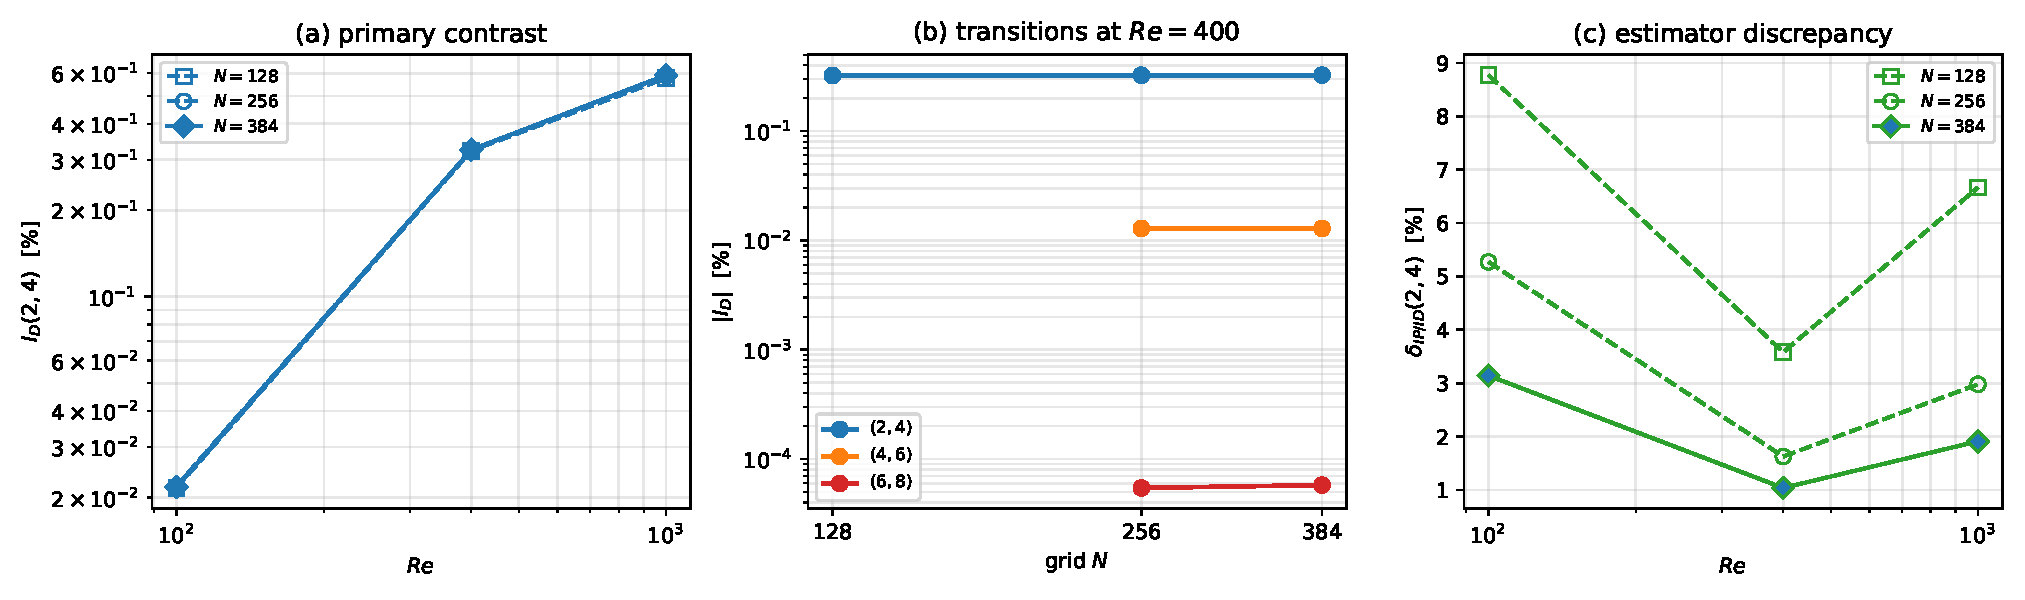
\includegraphics[width=0.85\columnwidth]{figures/figS_contrasts_res.pdf}
\caption{Resolution dependence at $\alpha=0$, with $N=384$ included in every series (open markers). (a) Primary contrast $I_D(2,4)$ for $Re=100$, $400$, $1000$. (b) All three successive transitions at $Re=400$ and $Re=1000$, the two Reynolds numbers for which $(4,6)$ and $(6,8)$ were computed; logarithmic ordinate. (c) Estimator discrepancy $\delta_{IP/ID}(2,4)$ for the three Reynolds numbers. No series contains missing or extrapolated $N=384$ points.}
\label{suppfig:contrasts_res}
\end{figure}

\subsection{Spatial decomposition of the geometric contrast}

The global contrast between $n=4$ and $n=2$ is localized exactly by partitioning the $n=4$ fluid region into the part $A$ common to both geometries and the part $B$ added by flattening. Writing $\ell$ for the local dissipation density times the cell area, the identity
\begin{equation}
\Delta D=D^*(4,0)-D^*(2,0)=\underbrace{\sum_{A}(\ell_4-\ell_2)}_{\mathrm{d}A}+\underbrace{\sum_{B}\ell_4}_{\mathrm{d}B}
\end{equation}
holds cell by cell, because $A$ and $B$ are disjoint and their union is the whole $n=4$ region. The two terms and their sum are listed in Table~\ref{supptab:layers}; the sum $\mathrm{d}A+\mathrm{d}B$ reproduces the headline contrast $I_D(2,4)$ to machine precision, and the four bands of the common region (lid, bottom, side/corner, interior core) are disjoint and sum to $\mathrm{d}A$ exactly. The interior core is negative at all three $Re$; the lid and bottom bands are positive for $Re\ge400$ and weakly negative at $Re=100$, where the largest common-region contribution is the side/corner band. The added-region term $\mathrm{d}B$ is positive at all $Re$ and grows monotonically. The redistribution term $\mathrm{d}A$ is negative only at $Re=100$ and crosses zero near $Re\approx145$ (Table~\ref{supptab:dadb}), so the net contrast $I_D(2,4)$ is positive at all Reynolds numbers while only $\mathrm{d}A$ changes sign.

\paragraph{Choice of band thresholds.}
The four-band decomposition of the common region $A$ uses thresholds chosen to isolate the physically distinct zones where dissipation concentrates or where the geometric change has its strongest effect. The \emph{lid band} (top $10\%$ of the cavity, $y>0.9$) captures the shear layer driven by the moving lid, which contains $74$--$84\%$ of the total dissipation depending on $Re$ (Section~IV.C of the main text). The \emph{bottom band} (below $y_b+0.1$, where $y_b(x)$ is the bottom-wall height) isolates the near-wall region directly affected by the superelliptic shaping; at $0.1$ in wall distance it extends just far enough above the bottom to capture the wall-normal dissipation gradient without overlapping the core. The \emph{side/corner zone} (within $0.1$ of any vertical wall) captures the lateral boundary layers and the rounded-corner fillets where the Bouzidi treatment resolves the curved geometry. The \emph{interior core} is the remainder: the bulk recirculation zone away from all walls. These thresholds ($10\%$, $0.1$) are not tuned to fit a particular result; they are round numbers of order $10\%$ that separate the cavity into its natural flow regions. A sensitivity test at $Re=400$ with alternative thresholds ($8\%$ and $12\%$ for the lid band, $0.08$ and $0.12$ for the bottom/side zones) changes the individual band contributions by at most $15\%$ but leaves the sum $\mathrm{d}A$ unchanged to machine precision (by construction, since the bands are disjoint and exhaustive) and the total contrast $I_D(2,4)$ identical. The physical interpretation---lid-dominated dissipation with a weakly dissipative added region---is therefore robust to the exact threshold values, which serve only to organize the accounting, not to determine it.

\begin{table}[!htbp]
\centering
\caption{Exact partition of the dissipation contrast $(n{=}4)-(n{=}2)$, $\alpha=0$, at $N=384$. All entries are in units of $10^{-4}D^*(2,0)$. The four bands of the common region $A$ are disjoint and sum to $\mathrm{d}A$; the added region $B$ gives $\mathrm{d}B$; their sum is $\Delta D$ and equals the headline contrast $I_D(2,4)$. Lid band: top $10\%$; bottom band: below $y_b+0.1$; side/corner: within $0.1$ of a vertical wall; core: the remainder.}
\label{supptab:layers}
\begin{tabular}{@{}lccc@{}}
\hline
Region & $Re=100$ & $Re=400$ & $Re=1000$ \\
\hline
Lid band (top $10\%$)         & $-1.33$ & $+24.42$ & $+55.51$ \\
Bottom band (below $y_b{+}0.1$)& $-1.29$ & $+6.21$ & $+23.07$ \\
Side/corner zone              & $+7.13$ & $+10.44$ & $-2.17$ \\
Interior core                 & $-9.33$ & $-28.29$ & $-65.97$ \\
\hline
$\mathrm{d}A$ (sum of bands)  & $-4.81$ & $+12.78$ & $+10.44$ \\
$\mathrm{d}B$ (added region)  & $+6.99$ & $+19.71$ & $+48.65$ \\
\hline
$\Delta D=\mathrm{d}A+\mathrm{d}B$ & $+2.18$ & $+32.49$ & $+59.09$ \\
$I_D(2,4)$ [\%]               & $+0.0218$ & $+0.3249$ & $+0.5909$ \\
\hline
\end{tabular}
\end{table}

Table~\ref{supptab:dadb} follows $\mathrm{d}A$ and $\mathrm{d}B$ along the $N=128$ Reynolds sweep. The added-region term $\mathrm{d}B$ increases monotonically throughout, whereas $\mathrm{d}A$ is negative at $Re=100$, crosses zero between $Re=100$ and $Re=150$, reaches a maximum near $Re=600$, and then decreases slowly. The two terms therefore have genuinely different Reynolds dependence, which is what makes the contrast non-power-law: $\mathrm{d}B$ grows roughly linearly in $Re$ while $\mathrm{d}A$ saturates and turns over.

\begin{table}[!htbp]
\centering
\caption{Partition $\mathrm{d}A$, $\mathrm{d}B$ and their sum along the $N=128$ Reynolds sweep, $\alpha=0$, in units of $10^{-4}D^*(2,0)$. The redistribution $\mathrm{d}A$ changes sign near $Re\approx145$.}
\label{supptab:dadb}
\begin{tabular}{@{}r|rrr@{\hskip 18pt}r|rrr@{}}
\hline
$Re$ & $\mathrm{d}A$ & $\mathrm{d}B$ & $\Delta D$ & $Re$ & $\mathrm{d}A$ & $\mathrm{d}B$ & $\Delta D$ \\
\hline
100 & $-4.73$ & $+6.89$ & $+2.16$ & 600 & $+15.62$ & $+28.21$ & $+43.83$ \\
150 & $+0.74$ & $+7.76$ & $+8.50$ & 650 & $+15.56$ & $+30.51$ & $+46.08$ \\
200 & $+4.91$ & $+9.37$ & $+14.28$ & 700 & $+15.39$ & $+32.74$ & $+48.14$ \\
250 & $+8.16$ & $+11.37$ & $+19.53$ & 750 & $+15.13$ & $+34.91$ & $+50.04$ \\
300 & $+10.63$ & $+13.63$ & $+24.26$ & 800 & $+14.80$ & $+37.00$ & $+51.80$ \\
350 & $+12.46$ & $+16.02$ & $+28.48$ & 850 & $+14.41$ & $+39.03$ & $+53.44$ \\
400 & $+13.76$ & $+18.49$ & $+32.25$ & 900 & $+13.98$ & $+40.99$ & $+54.97$ \\
450 & $+14.65$ & $+20.97$ & $+35.62$ & 950 & $+13.52$ & $+42.89$ & $+56.41$ \\
500 & $+15.21$ & $+23.43$ & $+38.64$ & 1000 & $+13.03$ & $+44.73$ & $+57.76$ \\
550 & $+15.51$ & $+25.85$ & $+41.36$ & & & & \\
\hline
\end{tabular}
\end{table}

\begin{table}[!htbp]
\centering
\caption{Grid robustness of the spatial partition $\mathrm{d}A/\mathrm{d}B$ for the primary contrast $(2,4)$ at $\alpha=0$, in units of $10^{-4}D^*(2,0)$. The four bands of the common region $A$ (lid, bottom, side/corner, core) are disjoint and sum to $\mathrm{d}A$; the added region $B$ gives $\mathrm{d}B$; their sum is $\Delta D = \mathrm{d}A + \mathrm{d}B$ and equals the headline contrast $I_D(2,4)$. Every resolution is evaluated cell by cell with the \emph{same} exact method; the $N=384$ rows reproduce Table~\ref{supptab:layers} to machine precision, so no interpolation or change of estimator is involved. The cancellation index $C=\sum|\text{bands}|/|\mathrm{d}A|$ measures the degree of internal cancellation within $\mathrm{d}A$. $N=512$ was not run at $Re=100$. The sign and order of magnitude of $\mathrm{d}A$ and $\mathrm{d}B$ are stable across all grids; the individual band magnitudes carry a grid sensitivity of up to $\sim 27\%$ at $Re=1000$, which largely cancels in $\Delta D$, whose uncertainty remains $\leq2.4\%$ of its value.}
\label{supptab:dadb_multires}
\footnotesize
\begin{tabular}{@{}cc|cccc|cccc@{}}
\hline
$Re$ & $N$ & lid & bottom & side & core & $\mathrm{d}A$ & $\mathrm{d}B$ & $\Delta D$ & $C$ \\
\hline
$100$  & $128$ & $-1.47$ & $-1.16$ & $+7.12$ & $-9.23$ & $-4.73$  & $+6.89$  & $+2.16$  & $4.0$ \\
       & $256$ & $-1.44$ & $-1.28$ & $+7.01$ & $-9.11$ & $-4.82$ & $+7.01$ & $+2.19$ & $3.9$ \\
       & $384$ & $-1.33$ & $-1.29$ & $+7.13$ & $-9.33$ & $-4.81$ & $+6.99$ & $+2.18$ & $4.0$ \\
\hline
$400$  & $128$ & $+24.48$ & $+6.55$ & $+10.22$ & $-27.48$ & $+13.76$ & $+18.49$ & $+32.25$ & $5.0$ \\
       & $256$ & $+24.36$ & $+6.18$ & $+10.27$ & $-27.88$ & $+12.91$ & $+19.55$ & $+32.46$ & $5.3$ \\
       & $384$ & $+24.42$ & $+6.21$ & $+10.44$ & $-28.29$ & $+12.78$ & $+19.71$ & $+32.49$ & $5.4$ \\
       & $512$ & $+24.34$ & $+6.18$ & $+10.41$ & $-28.23$ & $+12.71$ & $+19.78$ & $+32.49$ & $5.4$ \\
\hline
$1000$ & $128$ & $+55.90$ & $+23.92$ & $-2.61$ & $-64.19$ & $+13.03$ & $+44.73$ & $+57.76$ & $11.3$ \\
       & $256$ & $+55.43$ & $+22.84$ & $-2.53$ & $-64.99$ & $+10.75$ & $+48.02$ & $+58.77$ & $13.6$ \\
       & $384$ & $+55.51$ & $+23.07$ & $-2.17$ & $-65.97$ & $+10.44$ & $+48.65$ & $+59.09$ & $14.1$ \\
       & $512$ & $+55.39$ & $+23.05$ & $-2.26$ & $-65.96$ & $+10.22$ & $+48.95$ & $+59.18$ & $14.3$ \\
\hline
\end{tabular}
\end{table}

\begin{figure}[!htbp]
\centering
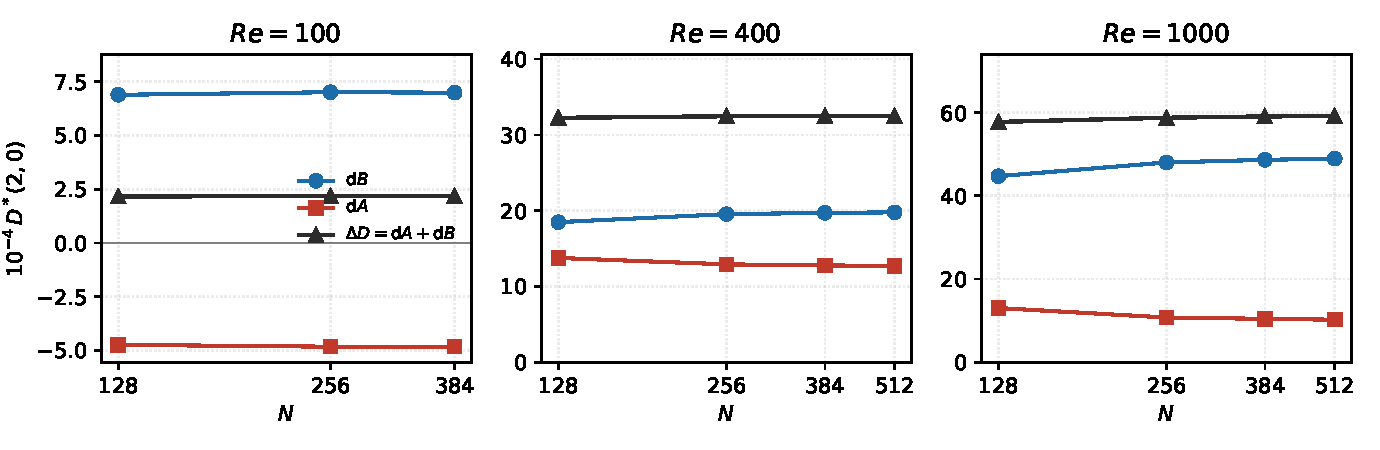
\includegraphics[width=0.98\columnwidth]{figures/figS_dadb_res.pdf}
\caption{Resolution dependence of the exact $\mathrm{d}A/\mathrm{d}B$ partition of the $(2,4)$ contrast at $\alpha=0$, in units of $10^{-4}D^*(2,0)$, computed cell by cell with the same method on each grid. The added-region term $\mathrm{d}B$ (circles) and the common-region redistribution $\mathrm{d}A$ (squares) are individually grid-sensitive --- $\mathrm{d}A$ varies by up to $\sim27\%$ at $Re=1000$ --- but their sum $\Delta D=\mathrm{d}A+\mathrm{d}B$ (triangles), which equals $I_D(2,4)$, is stable to within $2.4\%$ across all grids. $N=512$ was not run at $Re=100$.}
\label{suppfig:dadb_res}
\end{figure}

All entries in Table~\ref{supptab:dadb_multires} are recomputed from the stored velocity fields with the identical exact-partition code, so the $N=384$ rows reproduce Table~\ref{supptab:layers} to machine precision and the four bands are now available at \emph{every} resolution, including $N=128$ (which an earlier partial computation had left incomplete). The cancellation index $C$ increases both with $Re$ and, at fixed $Re$, with refinement: $4.0$ ($Re=100$), $5.0\to5.4$ ($Re=400$), and $11.3\to14.3$ ($Re=1000$) from $N=128$ to $N=512$, reflecting the growing internal cancellation within $\mathrm{d}A$ as the lid and core bands become larger and more opposed. Despite this, the net contrast $\Delta D = \mathrm{d}A + \mathrm{d}B$ --- and therefore $I_D(2,4)$ --- remains stable to within $2.4\%$ of its value across $N=128$--$512$ at all three Reynolds numbers, because the grid-induced changes in $\mathrm{d}A$ and $\mathrm{d}B$ partially cancel (Fig.~\ref{suppfig:dadb_res}).

\paragraph{Two-level interpretation of the mechanism.}
The $\mathrm{d}A/\mathrm{d}B$ decomposition supports two levels of conclusion, with different robustness to grid resolution:

\emph{Robust (qualitative) level:} (i)~The sign of $\mathrm{d}B$ is positive at all $Re$ and all $N$, confirming that the newly opened shoulder region always adds dissipation. (ii)~The sign of $\mathrm{d}A$ is negative at $Re=100$ and positive at $Re\geq 400$, confirming that the common-region redistribution changes sign near $Re\approx 145$. (iii)~The magnitude of $\mathrm{d}B$ is comparable to or larger than $\Delta D$, confirming that the sub-extensive response arises from a near-cancellation between $\mathrm{d}A$ and $\mathrm{d}B$. (iv)~The dissipation is concentrated in the lid band at $Re\geq 400$, where it accounts for $74$--$84\%$ of the total.

\emph{Quantitative level:} The individual magnitudes of the four bands and of $\mathrm{d}A$ carry a grid sensitivity that grows with $Re$: $\mathrm{d}A$ spans $0.09$ units ($1.9\%$ of itself) at $Re=100$, $1.05$ units ($8.2\%$) at $Re=400$, and $2.81$ units ($27\%$) at $Re=1000$ across $N=128$--$512$. This is the price of the internal cancellation, quantified by the rising index $C$. The sensitivity does not contaminate the net contrast $\Delta D$, whose grid dependence is bounded by $2.4\%$ across $N=128$--$512$. The quantitative mechanism---the exact balance between lid-band gain and core-band loss---is therefore best resolved at the finer grids ($N\ge256$, where the band values have settled to within a few percent), while the coarse $N=128$ bands should be read as order-of-magnitude estimates rather than converged values.

\paragraph{Alternative two-zone decomposition.}
To test whether the four-band split is essential to the conclusion, we define an alternative \emph{near-wall} zone (lid $+$ bottom $+$ side bands) and \emph{bulk} zone (core band). At $Re=400$, $N=384$, this gives $\mathrm{d}A_{\text{near-wall}} = +41.07$ and $\mathrm{d}A_{\text{bulk}} =-28.29$, with $C_{\text{alt}} = (41.07 + 28.29)/12.78 = 5.4$ (identical to the four-band $C$ by construction, since the bands are merely regrouped). The net $\mathrm{d}A = +12.78$ is unchanged. At $Re=1000$, $\mathrm{d}A_{\text{near-wall}} = +76.41$ and $\mathrm{d}A_{\text{bulk}} = -65.97$, giving $\mathrm{d}A = +10.44$ and $C_{\text{alt}} = 14.1$. The qualitative conclusion---that $\mathrm{d}A$ is a near-cancellation between opposing near-wall and bulk contributions---is therefore independent of the four-band split; the split serves only to localize the cancellation within the near-wall region (between lid, bottom, and side) and the bulk (core).

\begin{figure}[!htbp]
\centering
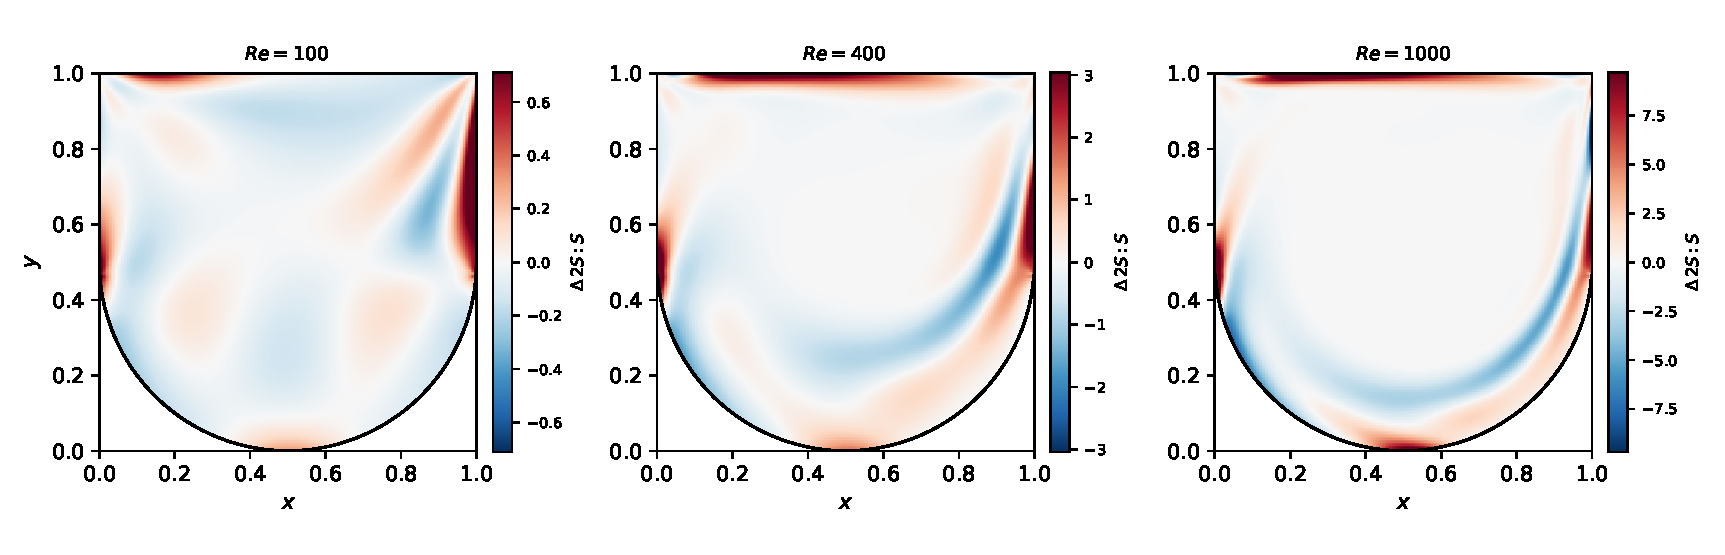
\includegraphics[width=0.98\columnwidth]{figures/figS_deltaD_maps.pdf}
\caption{Local dissipation contrast $\Delta(2\mu\mathbf{S}{:}\mathbf{S})=(n{=}4)-(n{=}2)$ at $\alpha=0$, $N=384$, evaluated on the $n=2$ region, for $Re=100$, $400$, $1000$. The lid and bottom bands are positive at $Re\ge400$ and weakly negative at $Re=100$, the interior core is negative throughout, and the net contrast $I_D(2,4)$ remains positive at all three Reynolds numbers.}
\label{suppfig:deltaD}
\end{figure}

\subsection{Reynolds-number sweep}

The exploratory parameter sweep at $N=128$, with complete LBM parameters recorded in Table~\ref{supptab:resweep_params}, resolves the continuous variation of the primary contrast $I_D(2,4)$ at $\alpha=0$ (Table~\ref{supptab:resweep}). The local logarithmic slope $\gamma_{\rm loc}=d\ln|I_D|/d\ln Re$ decreases monotonically from $2.72$ near $Re=150$ to $0.47$ near $Re=950$ (the central-difference estimate ends one interval before the largest $Re$), crossing unity near $Re\approx346$. As discussed in the main text, this smooth inflection reflects the competition between the linear growth of the added-region dissipation and the saturation of common-region redistribution; the value $Re\approx346$ is reported as a descriptive feature of this coarse-grid trajectory, not an exact universal scaling law.

\begin{table}[!htbp]
\centering
\caption{Primary contrast $I_D(2,4)$ at $\alpha=0$ from the $N=128$ exploratory Reynolds sweep.}
\label{supptab:resweep}
\begin{tabular}{@{}cc|cc@{}}
\hline
$Re$ & $I_D$ [\%] & $Re$ & $I_D$ [\%] \\
\hline
100 & 0.02160 & 150 & 0.08500\\
200 & 0.14280 & 250 & 0.19534\\
300 & 0.24259 & 350 & 0.28482\\
400 & 0.32251 & 450 & 0.35619\\
500 & 0.38640 & 550 & 0.41363\\
600 & 0.43829 & 650 & 0.46078\\
700 & 0.48139 & 750 & 0.50038\\
800 & 0.51798 & 850 & 0.53437\\
900 & 0.54968 & 950 & 0.56405\\
1000 & 0.57758 & \\
\hline
\end{tabular}
\end{table}

\subsection{Robustness tests}

\emph{Wall-gradient treatment.} Replacing the geometric wall-distance correction of the bottom-wall one-sided gradient by a purely node-based one-sided difference changes $I_D(2,4)$ from $0.0218\%$ to $0.0207\%$ ($Re=100$), $0.3249\%$ to $0.3212\%$ ($Re=400$), and $0.5909\%$ to $0.5777\%$ ($Re=1000$); the contrast changes by $5.0\%$ of its own value at $Re=100$ and by only $1.1$--$2.2\%$ at $Re=400$--$1000$.

\emph{Effective-Reynolds perturbation.} A $0.4\%$ differential shift of the effective Reynolds number between the two geometries propagates to a change of $0.0005\%$ in $I_D(2,4)$ at $Re=100$ ($2\%$ of its value) and $0.0011\%$ at $Re=400$ ($0.4\%$).

\emph{Grid span.} Because the residual change between the two finest grids is dominated by the partial cancellation of common discretization error rather than by a clean power-law decay, no Richardson extrapolation or GCI is quoted; the span of $I_D(2,4)$ over $N=128$--$384$ is taken as the conservative numerical uncertainty: $3.4\times10^{-4}$ percentage points ($Re=100$), $2.4\times10^{-3}$ ($Re=400$), $1.3\times10^{-2}$ ($Re=1000$), i.e.\ at most $2.3\%$ of the finest-grid contrast.

\emph{Discrete versus analytic area.} The discrete fluid area differs from the analytic value of \texttt{area\_fluid} by at most $0.017\%$ over all cases, so the choice of discrete or analytic reference area does not affect any quoted contrast.
